\documentclass[aspectratio=1610]{beamer}
\usetheme{Madrid}
\usecolortheme{default}
\useoutertheme{split}
\useinnertheme{circles}
\usepackage{xcolor}
\usepackage{mathrsfs}
\usepackage{amsmath}
\usepackage{amssymb}
\usepackage{booktabs}
\usepackage{hyperref}
\usepackage{graphicx}
\usepackage{caption}
\captionsetup[figure]{font=tiny}

% --- Couleurs CS ---
\definecolor{CSred}{RGB}{160,32,60}
\definecolor{CSgrey}{RGB}{136,121,150}
\definecolor{UPSred}{RGB}{97,21,58}
\setbeamercolor{titlelike}{bg=CSred}
\setbeamerfont{title}{series=\bfseries}
\setbeamercolor{palette primary}{bg=CSred,fg=white}
\setbeamercolor{palette secondary}{bg=CSred,fg=white}
\setbeamercolor{palette tertiary}{bg=CSgrey,fg=white}
\setbeamercolor{palette quaternary}{bg=CSgrey,fg=white}
\setbeamercolor{structure}{fg=CSgrey}

\title[Radiomics \& Immunotherapy]{Critical Appraisal: A Radiomics Approach to Assess Tumour-Infiltrating CD8 Cells and Response to Anti-PD-1/PD-L1 Immunotherapy}
\subtitle{Sun et al., \textit{The Lancet Oncology}, 2018}
\author[CORCOS, JAMAL, MARTINI]{Ethan CORCOS, Adonis JAMAL, Jean-Vincent MARTINI}
\institute[]{MVA \& MSV - Biostatistics}
\date{March 17, 2026}

\begin{document}

\frame{\titlepage}

% ==============================================================================
% SECTION 1: BACKGROUND
% ==============================================================================
%\section{Background}

% \begin{frame}{Background — Methodological Topic}
%     \begin{block}{Radiomics}
%         \textbf{Radiomics} = computational analysis of medical images to extract high-dimensional quantitative features (texture, shape, intensity) from tumours
%         \begin{itemize}
%             \item Hypothesis: imaging reflects not only macroscopic but also \textit{cellular and molecular} tissue properties
%             \item Non-invasive, enables whole-tumour and microenvironment characterisation
%             \item Here: combined with \textbf{RNA-seq genomics} and \textbf{machine learning} to build an imaging biomarker
%         \end{itemize}
%     \end{block}
%     \begin{alertblock}{ML / AI Component}
%         \begin{itemize}
%             \item Supervised regression from image features $\rightarrow$ genomic CD8 score
%             \item Feature selection via \textbf{elastic-net regularised regression}
%         \end{itemize}
%     \end{alertblock}
% \end{frame}

\begin{frame}{Background: Medical Problem \& Importance}
    \begin{columns}[T]
        \begin{column}{0.55\textwidth}
            \textbf{Problem:} Predicting response to cancer immunotherapy
            \begin{itemize}
                \item Anti-PD-1 / anti-PD-L1 checkpoint inhibitors have transformed oncology (melanoma, lung, lymphoma\ldots)
                \item \textbf{Only 20-50\%} of patients with advanced solid tumours respond to treatment
                \item Need to identify \textit{a priori} which patients will benefit
            \end{itemize}
            \vspace{0.3em}
            \textbf{Known biology:} Pre-existing tumour immune infiltration by \textbf{CD8+ cytotoxic T cells} correlates with response to PD-1/PD-L1 therapy
        \end{column}
        \begin{column}{0.42\textwidth}
            \begin{exampleblock}{Three Immune Phenotypes}
                \begin{itemize}
                    \item \textcolor{green!60!black}{\textbf{Immune-inflamed}}: dense CD8 infiltrate, responds to immunotherapy
                    \item \textbf{Immune-excluded}: T cells blocked at tumour periphery
                    \item \textcolor{red}{\textbf{Immune-desert}}: low CD8 infiltrate, poor response
                \end{itemize}
            \end{exampleblock}
        \end{column}
    \end{columns}
\end{frame}

\begin{frame}{Background: State of the Art \& Limitations}
    \begin{block}{State of the Art at Time of Publication}
        \begin{itemize}
            \small
            \item CD8 infiltration assessed by \textbf{immunohistochemistry (IHC)} or \textbf{RNA sequencing} from tumour biopsies
            \item \textbf{PD-L1 expression} used as a biomarker but two RCTs showed it was \textit{not} reliably associated with response
            \item 4 published studies explored radiomics and immune infiltration, but:
                \begin{itemize}
                    \item No patients treated with immunotherapy
                    \item Only \textit{one} had an external validation cohort
                    \item Evidence level remained low
                \end{itemize}
        \end{itemize}
    \end{block}
    \begin{alertblock}{Limitations of Existing Approaches}
        \begin{itemize}
            \small
            \item Biopsies are \textbf{invasive}, spatially limited (sampling bias), and not repeatable
            \item Cannot capture \textbf{spatial heterogeneity} or longitudinal changes
            \item No validated imaging-based predictor of immunotherapy response existed
        \end{itemize}
    \end{alertblock}
\end{frame}

% ==============================================================================
% SECTION 2: OBJECTIVES & CONTRIBUTIONS
% ==============================================================================
%%%\section{Objectives \& Contributions}

\begin{frame}{Objectives \& Main Contributions}
    \begin{block}{Objective}
        Develop and independently validate a \textbf{CT-based radiomic signature of tumour-infiltrating CD8 cells}, and evaluate its ability to predict tumour immune phenotype and clinical outcomes in patients treated with anti-PD-1/PD-L1 immunotherapy.
    \end{block}

    \begin{block}{Main Contributions}
        \begin{enumerate}
            \item \textbf{First} radiomics-based biomarker of CD8 tumour infiltration validated in \textit{three} independent cohorts
            \item Link demonstrated between CT texture features and \textbf{gene expression}, \textbf{pathology}, and \textbf{clinical response}
            \item Radiomic score shown to be \textbf{independent prognostic factor} for overall survival under immunotherapy
        \end{enumerate}
    \end{block}
\end{frame}


% ==============================================================================
% SECTION 3: METHODOLOGY
% ==============================================================================
%%%\section{Methodology}

\begin{frame}{Methodology: Segmentation \& Feature Extraction}
    \begin{columns}
        \begin{column}{0.6\textwidth}
            \small
            \textbf{Two Volumes of Interest (VOIs):}
            \begin{enumerate}
                \small
                \item \textbf{Tumour}: semi-automatically delineated by 3 radiation oncologists (ISOgray v4.1)
                \item \textbf{Peripheral ring}: automated $\pm 2$ mm dilation/shrinkage of tumour boundary (4 mm ring)
            \end{enumerate}
       
            \textit{Motivation for ring: capture the tumour \textbf{microenvironment}, where immune cells infiltrate from periphery}\\

            \textbf{Features extracted:}
            \begin{itemize}
                \small
                \item 4 grey-level matrices (3D): GLRLM, etc.
                \item 39 features per VOI $\rightarrow$ \textbf{78 radiomic features}
                \item + 5 location variables + 1 technical variable (kVp)
                \item \textbf{Total: 84 input variables}
            \end{itemize}
        \end{column}
        \begin{column}{0.4\textwidth}
            \begin{alertblock}{Why include kVp (peak kilovoltage)?}
                Textural features are \textbf{highly dependent} on image acquisition parameters. Including kVp corrects for inter-scanner variability in heterogeneous cohorts.
            \end{alertblock}
            \begin{exampleblock}{Why include VOI location?}
                Tissue origin has a major effect on tumour immune contexture: liver vs. adenopathy vs. lung lesions have different baseline textures.
            \end{exampleblock}
        \end{column}
    \end{columns}
\end{frame}

\begin{frame}{Methodology: Response Variable \& Machine Learning}
    \begin{block}{Response Variable: CD8 Gene Expression Signature}
        \begin{itemize}
            \footnotesize
            \item \textbf{MOSCATO}: RNA-seq quantified with Salmon (\textbf{TPM}); \textbf{TCGA}: quantified as \textbf{RPKM} (different methods, corrected only by mean/variance rescaling
            \item CD8 abundance estimated via \textbf{CD8B gene signature} (Becht et al., MCPcounter)); log$_2$-transformed, binarised at the \textbf{median} for AUC computation
        \end{itemize}
    \end{block}

    \begin{alertblock}%{PROBAST D3 — Surrogate Outcome}
        \footnotesize
        CD8B gene expression is a \textbf{computational surrogate}, not a direct measurement of CD8 cell infiltration. The full inference chain is: \textit{imaging $\rightarrow$ gene expression $\rightarrow$ assumed CD8 count $\rightarrow$ clinical response}. Each link is an untested assumption.
    \end{alertblock}

    \begin{block}{Elastic-Net Regularised Regression}
        $$\hat{y} = a_1 X_1 + \cdots + a_i X_i + b$$
        \vspace{-0.5cm}
        \begin{itemize}
            \footnotesize
            \item L1 (lasso) $+$ L2 (ridge) penalties: simultaneous \textbf{feature selection} and \textbf{coefficient shrinkage}
            \item $\alpha = 0.5$ (grid search), $\lambda$ by cross-validation; \textbf{8 variables retained} from 84
        \end{itemize}
        %% https://glmnet.stanford.edu/articles/glmnet.html
    \end{block}
\end{frame}

\begin{frame}{Methodology: The 8-Variable Radiomic Signature}
    \small
    \begin{columns}[T]
        \begin{column}{0.55\textwidth}
            The elastic-net retained:
            \begin{itemize}
                \small
                \item \textbf{5 radiomic features}:
                    \begin{itemize}
                        \item 1 first-order feature
                        \item 4 second-order features from the \textbf{Grey-Level Run Length Matrix (GLRLM)}
                    \end{itemize}
                \item \textbf{2 VOI location} variables: adenopathy, head \& neck
                \item \textbf{1 technical variable}: peak kilovoltage
            \end{itemize}
            \vspace{-0.2cm}
            \begin{exampleblock}{Intuitive interpretation}
                \small
                \textit{Relatively \textbf{homogeneous, hypodense} tumours and peripheral rings} were associated with a \textbf{high CD8 score}, consistent with inflammatory infiltrate. Heterogeneity/high grey levels may reflect necrosis or chaotic vascularisation
            \end{exampleblock}
        \end{column}
        \begin{column}{0.42\textwidth}
            \begin{alertblock}{GLRLM: Why?}
                The \textbf{Grey-Level Run Length Matrix} quantifies texture \textit{homogeneity/heterogeneity} i.e., how far uniform intensity values extend in a given direction. It captures the spatial structure of immune infiltrate patterns.
            \end{alertblock}
            \vspace{0.3em}
            \begin{alertblock}{Critical Note}
                Only \textbf{8 of 84} variables retained: strong regularisation avoids overfitting but may also discard relevant features.
            \end{alertblock}
        \end{column}
    \end{columns}
\end{frame}

% ==============================================================================
% SECTION 4: VALIDATION & RESULTS
% ==============================================================================
%%%\section{Validation \& Results}

\begin{frame}{Validation Strategy}
    \vspace{-0.3cm}
    \begin{block}{Four-Cohort Design}
        \footnotesize
        \begin{tabular}{lll}%{p{3.2cm}p{2.5cm}p{4.5cm}}
            \toprule
            \textbf{Cohort} & \textbf{Endpoint} & \textbf{Rationale} \\
            \midrule
            MOSCATO ($n=135$) & AUC (\textbf{training}) & Build radiomic signature vs. CD8B RNA-seq \\
            TCGA/TCIA ($n=119$) & AUC (primary) & External genomic concordance in 5 cancer types \\
            Immune phenotype ($n=100$) & AUC & Inflamed vs. desert tumours (extreme phenotypes) \\
            Immunotherapy cohort ($n=137$) & ORR, OS, PFS & Clinical predictive/prognostic value \\
            % \bottomrule
        \end{tabular}
    \end{block} 
    \vspace{-0.3cm}
    \begin{columns}[T]
        \begin{column}{0.48\textwidth}
            \small
            \begin{exampleblock}{Strengths}
                \begin{itemize}
                    \item 3 truly \textit{independent} val. cohorts
                    \item Statistically different cohorts $\Rightarrow$ no overfitting to a tumour subset
                    \item Pathologist masked to radiomic results
                \end{itemize}
            \end{exampleblock}
        \end{column}
        \begin{column}{0.48\textwidth}
            \begin{alertblock}{Limitations}
                \begin{itemize}
                    \item All cohorts retrospective
                    \item TCGA: strict QC $\Rightarrow$ only 119/435 eligible
                    \item Immune phenotype: labels defined by \textbf{tumour type} (e.g., melanoma $=$ inflamed), not pathological confirmation $\rightarrow$ \textit{circular} with the downstream clinical claim
                \end{itemize}
            \end{alertblock}
        \end{column}
    \end{columns}
\end{frame}

\begin{frame}{Key Results: Radiomic Signature Performance}
    \begin{columns}[T]
        \begin{column}{0.5\textwidth}
            \begin{block}{AUC Results (High vs. Low CD8)}
                \begin{itemize}
                    \item \textbf{MOSCATO training}: AUC = 0.74 (0.66--0.82), $p < 0.0001$
                    \item \textbf{TCGA validation}: AUC = 0.67 (0.57--0.77), $p = 0.0019$
                    \item \textbf{Immune phenotype}: AUC = 0.76 (0.66--0.86), $p < 0.0001$
                \end{itemize}
            \end{block}
            \begin{block}{Pathology Concordance (TCGA)}
                Spearman $\rho = 0.559$, $p = 0.00022$ (4 cancer types \textbf{pooled}: BLCA, LUAD, LUSC, LIHC; $n=39$)\\
                \textit{Not significant for HNSC ($p=0.18$)}
            \end{block}
        \end{column}
        \begin{column}{0.48\textwidth}
            \begin{alertblock}{Critical Note on AUC}
                AUC of 0.67 in the TCGA validation set is \textbf{modest}: suggests limited discriminative power in a truly external, multi-centre, multi-cancer dataset. The authors acknowledge this is exploratory.
            \end{alertblock}
            \vspace{0.3em}
            \begin{exampleblock}{Sensitivity Analysis}
                Removing non-radiomic variables (kVp, VOI location) caused \textbf{worse} TCGA performance, confirming their necessity for heterogeneous cohorts.
            \end{exampleblock}
        \end{column}
    \end{columns}
\end{frame}

\begin{frame}{Key Results: Clinical Outcomes Under Immunotherapy}
    \begin{columns}[T]
        \begin{column}{0.35\textwidth}
            \small
            \textbf{Objective Response Rate}:
            \begin{itemize}
                \item At \textbf{3 months}: high score $\rightarrow$ higher ORR ($p=0.049$)
                \item At \textbf{6 months}: higher ORR ($p=0.025$) and disease control ($p=0.013$)
            \end{itemize}
            \vspace{0.3em}
            \textbf{Overall Survival ($n=137$):}
            \begin{itemize}
                \item Median OS: \textbf{24.3 vs 11.5 months}
                \item Univariate HR = 0.58 (0.39--0.87), $p=0.0081$
                \item \textbf{Multivariate} HR = 0.52 (0.35--0.79), $p=0.0022$
            \end{itemize}
            \vspace{0.3em}
            
        \end{column}
        \begin{column}{0.65\textwidth}
            \centering
            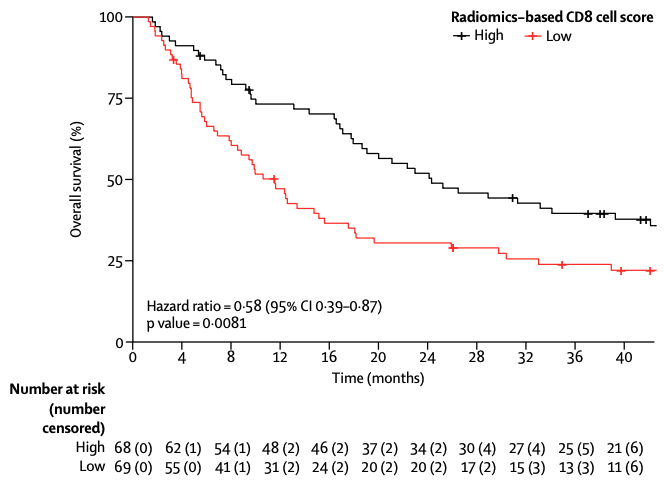
\includegraphics[width=0.8\linewidth]{img/overall_survival_sun_and_al.png}
            \captionof{figure}{\footnotesize Overall survival by radiomic score (high vs.\ low), Sun et al.\ 2018}
            \vspace{-0.3cm}
            \begin{alertblock}{}%{\small Critical Notes}
                \footnotesize
                \begin{itemize}
                    \item Median threshold: post-hoc, risks optimistic bias
                    \item All liver lesions $\rightarrow$ \textbf{low score group} (confounder)
                    \item 5 heterogeneous phase 1 trials
                \end{itemize}
            \end{alertblock}
        \end{column}
    \end{columns}
\end{frame}

% ==============================================================================
% SECTION 5: CONCLUSIONS
% ==============================================================================
%%%\section{Conclusions}

\begin{frame}{Conclusion}
    \begin{columns}[T]
        \begin{column}{0.48\textwidth}
            \begin{exampleblock}{Strengths}
                \begin{itemize}
                    \item Multi-cohort with 3 truly independent validation sets
                    \item Biologically motivated peripheral ring VOI
                    \item Elastic-net: principled feature selection
                    \item Sensitivity analysis confirming kVp/location necessity
                \end{itemize}
            \end{exampleblock}
        \end{column}
        \begin{column}{0.48\textwidth}
            \begin{alertblock}{Limitations}
                \begin{itemize}
                    \item Surrogate outcome (gene expression $\neq$ CD8 count); median binarisation
                    \item No \textbf{calibration} reported $\rightarrow$ discrimination (AUC) only
                    \item RPKM (TCGA) $\neq$ TPM (training) $\rightarrow$ quantification mismatch
                    \item Retrospective; median threshold post-hoc
                    \item Immune phenotype labels circular; liver lesion confounder
                    \item No prospective validation
                \end{itemize}
            \end{alertblock}
        \end{column}
    \end{columns}
\end{frame}

\begin{frame}{}
    \centering
    \LARGE
    \textbf{Thank you for your attention!}
\end{frame}

\begin{frame}{Appendix: Elastic-Net}
    \[
    \min_{\beta_0, \beta}\ \frac{1}{N}\sum_{i=1}^{N}\, l\!\left(y_i,\beta_0+\beta^T x_i\right)
    +\lambda \left[(1-\alpha)\|\beta\|_2^2/2+\alpha\|\beta\|_1\right]
    \]
    
    The Ridge penalty shrinks the coefficients of correlated predictors towards each other while the Lasso tends to pick one of them and discard the others. The elastic net penalty mixes these two: if predictors are correlated in groups, an $\alpha=0.5$ tends to either select or leave out the entire group of features.
\end{frame}

\begin{frame}{Appendix: Radiomics Workflow}
    \begin{figure}
        \centering
        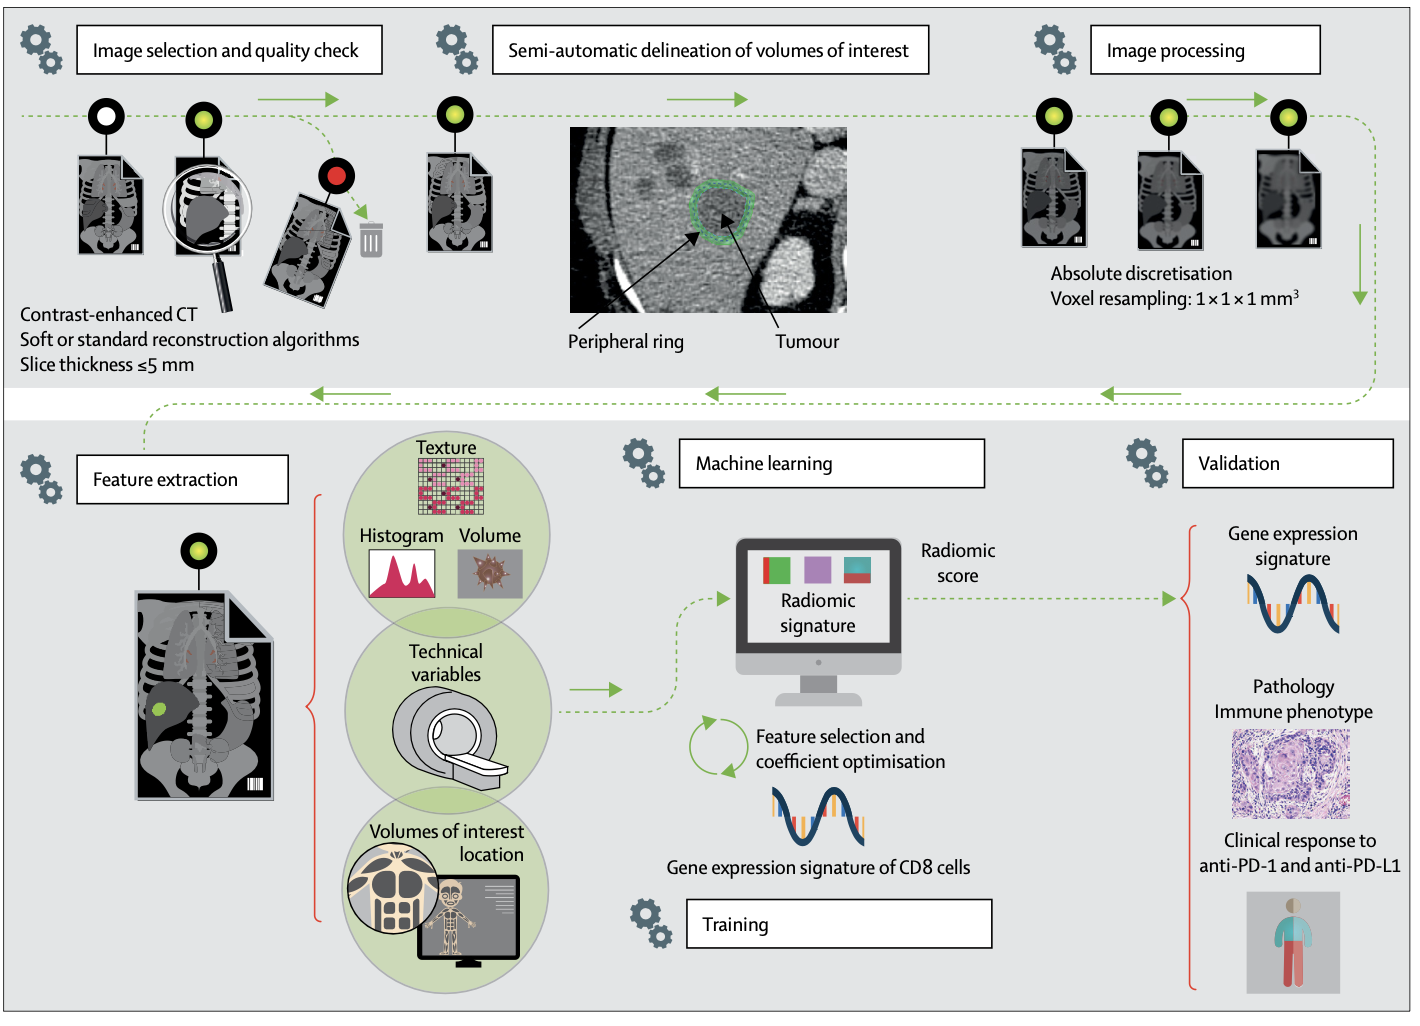
\includegraphics[width=0.7\linewidth]{image.png}
        \caption{Radiomics Workflow}
        \label{fig:placeholder}
    \end{figure}
\end{frame}

\end{document}